% Created 2022-11-11 Fri 12:34
% Intended LaTeX compiler: pdflatex
\documentclass[presentation,aspectratio=169]{beamer}
\usepackage[utf8]{inputenc}
\usepackage[T1]{fontenc}
\usepackage{graphicx}
\usepackage{grffile}
\usepackage{longtable}
\usepackage{wrapfig}
\usepackage{rotating}
\usepackage[normalem]{ulem}
\usepackage{amsmath}
\usepackage{textcomp}
\usepackage{amssymb}
\usepackage{capt-of}
\usepackage{hyperref}
\usepackage{pifont}
\newcommand{\cmark}{\textcolor{green!80!black}{\ding{51}}}
\usepackage{amssymb}
\usepackage{pgfplotstable}
\DeclareMathOperator{\shift}{q}
\DeclareMathOperator{\diff}{p}
\usepackage{khpreamble, euscript, mathtools}
\DeclareMathOperator{\atantwo}{atan2}
\newcommand*{\ctrb}{\EuScript{C}}
\newcommand*{\obsv}{\EuScript{O}}
\usetheme{default}
\author{Kjartan Halvorsen}
\date{\today}
\title{The Apollo LM state feedback assignment}
\hypersetup{
 pdfauthor={Kjartan Halvorsen},
 pdftitle={The Apollo LM state feedback assignment},
 pdfkeywords={},
 pdfsubject={},
 pdfcreator={Emacs 26.3 (Org mode 9.4.6)}, 
 pdflang={English}}
\begin{document}

\maketitle



\section{Apollo moon lander}
\label{sec:org356e4e4}

\begin{frame}[label={sec:org4981e16}]{The Apollo lunar module}
\begin{center}
  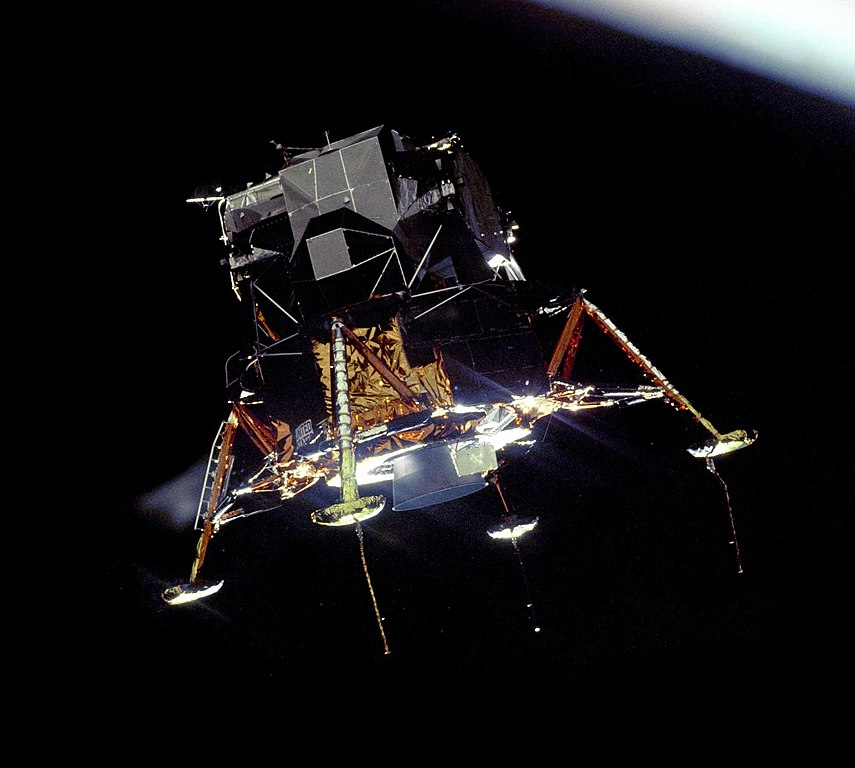
\includegraphics[width=0.5\linewidth]{../../figures/Apollo_11_Lunar_Module.jpg}
\end{center}
\end{frame}

\begin{frame}[label={sec:org65c426a}]{The Apollo lunar module}
\begin{center}
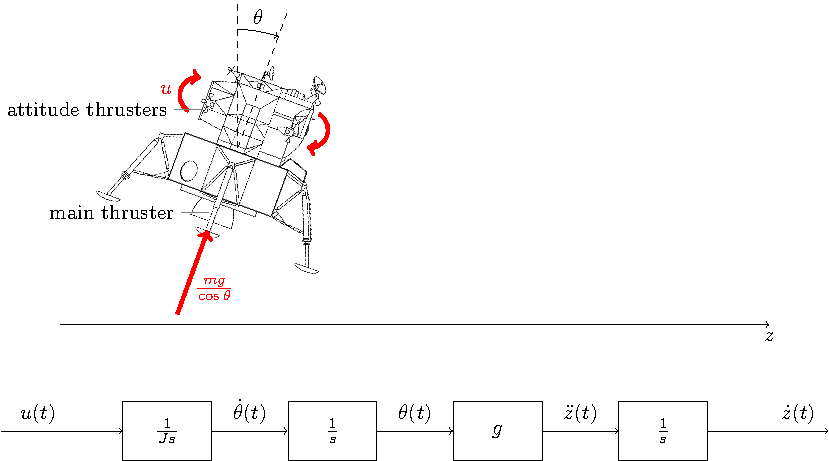
\includegraphics[width=0.7\linewidth]{../../figures/fig-apollo}
\end{center}

\pause

\alert{Activity} Which is the transfer function of the system?
   \[1: \; G(s) = \frac{\frac{g}{J} }{s^2}\qquad 2: \; G(s) = \frac{\frac{g}{J} }{s(s^2 + 1)} \qquad 3: \; G(s) = \frac{\frac{g}{J} }{s^3}\]
\end{frame}


\begin{frame}[label={sec:orgd1535e0}]{Plan}
\begin{enumerate}
\item Obtain discrete-time pulse transfer function for the LM.
\item Convert transfer function to discrete-time state space model.
\item Design a state feedback controller \(u(k) = Lx(k) + l_0r(k)\) to obtain good reference response.
\item Design an observer \(\hat{x}(k+1) = A\hat{x}(k) + B u(k) + K\big(y(k) - C\hat{x}(k)\big)\) and studying two cases: \alert{Slow observer vs fast observer.}
\end{enumerate}
\end{frame}


\begin{frame}[label={sec:org147d5b5}]{1. Discretize the continuous-time model}
\[ G(s) = \frac{\frac{g}{J} }{s^3}\]

The idea is to sample the continuous-time system's response to a step input, in order to obtain a discrete approximation which is \alert{exact} (at the sampling instants) for such an input signal. 

\begin{center}
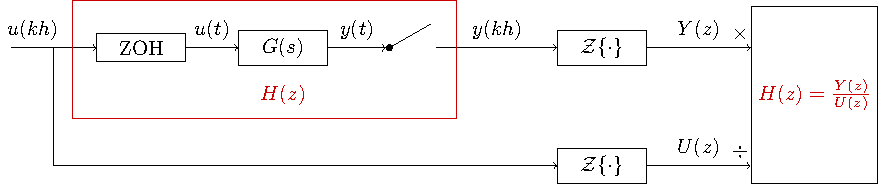
\includegraphics[width=0.9\linewidth]{../../figures/invariant-sampling.pdf}
\end{center}

Step-invariant sampling (zero order hold): \(u(kh) = \begin{cases} 1, & k \ge 0\\0, & k<0 \end{cases}\)
\end{frame}


\begin{frame}[label={sec:org34a31b1}]{2. Convert to discrete-time state space}
Using, for instance, the \alert{observable canonical form}

\begin{equation*}
H(z)=\frac{b_1z^{n-1}+\dots+b_{n-1}z+b_n}{z^n+a_1z^{n-1}+\dots
  +a_{n-1}z+a_n}
\end{equation*}
can be represented on state-space form as
\begin{align*}
x(k+1)&=\bbm -a_1& 1& 0 &\cdots &  0\\
-a_2 & 0& 1 &  \cdots& 0\\
-a_3 & 0 & 0& \cdots & 0\\
\vdots& \vdots& \vdots & \ddots& \vdots\\
-a_n& 0& 0 & \cdots& 0\ebm x(k) +
\bbm b_1\\ b_2\\ b_3\\ \vdots\\ b_n\ebm u(k)\\
y(k) &=\bbm 1& 0& \cdots& 0 \ebm x(k)
\end{align*}

\pause

\alert{Activity} Determine the discrete-time state-space model of the LM on observable canonical form
\end{frame}
\end{document}